\subsection{Greedy Heuristics Algorithm}
After having realised that even solving only a path optimal is very expensive, we will now interest ourselves with the notion of an approximation approach. The problem then becomes, which speed must we use for edges in a path, in the interval of $v_{min}$ and $v_{max}$. As argued previously, the optimal speed to drive can only be found by iterating over all possibilities which is a combinatorial optimization problem, and it is NP-Hard. Thus we must introduce a heuristic, which promotes local optimal choices. 

We will now analyse how to find this speed. Given a path $P = \langle u_1,u_2,\dots,u_k \rangle$. In measuring the fastest way to pass an edge on the path, there are two probable cases:
\begin{enumerate}
	\item It is fastest to drive
	\item It is fastest to charge, and then drive
\end{enumerate}

The intuition is then to figure out the time we will spend for both of these cases and picking the fastest option. However, it might not be possible to only drive, given the limited battery of the EV. The optimal speed when passing the edge $(u_i, u_j)$ without charging, can be found by solving this equation for $v$:
\[B_{cur} - D(u_i, u_j) * R_{CO}(v) = 0\] 
We call this speed $v_{opt}$. If $v_{opt}$ is lower than $v_{min}(e)$, the minimum speed of the edge, there is not enough energy in the battery to drive from $u_i$ to $u_j$ and thus the time is set to $-\infty$ indicating that just driving is not an option. If it is possible to drive the edge using the only energy from the battery the time it will take to pass the edge can be calculated as:
 \[T = \frac{D((u_i, u_j))}{v_{opt}} \] 
The time spent passing an edge $(u_i, u_j)$ while charging first, is given by the following equation:

\begin{equation*}
\begin{aligned}
 & T(v,(u_i, u_j)) = \frac{D((u_i, u_j))}{v} + \frac{R_{CO}(v) * D((u_i, u_j)) - B_{cur}}{charge_{rate}(u_j)}
\end{aligned}
\end{equation*}\label{eq:drivingAndCharging}

Where $v$ is the speed of the vehicle, $D(u_i, u_j)$ is the distance between vertices $u_i$ and $u_j$, $R_{CO}(v)$ is the consumption rate of the EV, $B_{cur}$ is the current battery of the vehicle. Since we only charge exactly enough to pass an edge, there might be charging stations previous to $u_i$ which we could have charged more at without exceeding the battery capacity. Thus we would go back in history and charge at the best previous charge stations, recursively, until we have enough energy to pass $(u_i, u_j)$ this is done by $charge_{rate}(u_i)$ which gives the charge rate of the best charge previous to $u_j$.

The above equation yields a function of the form: $av^2 + bv + c$, due to the fact that $R_{CO}(v)$ is a quadratic function. $a$, $b$ and $c$ are some constants which are given by the instance of the vehicle. Represented in a Cartesian coordinate system, $T(v,(u_i, u_j)))$ is a parabola, as can be seen in Figure \ref{fig:graph}, note that the graph is only defined for positive speeds larger than $0$ and can only be calculated if $charge_{rate}(u_j)$ is larger than $0$. On the x-axis is the speed of the vehicle and on the y-axis is the time spent. The turning point of the graph represents the optimal speed to drive for the given edge, denoted as $v_{opt}(e)$. The point is easily calculated by finding a tangent line with a slope of $0$. If $v_{opt}(e)$ is smaller than $v_{min}(e)$, then $v_{min}(e)$ defines the optimal speed for the edge. Similarly if $v_{opt}(e)$ is larger than $v_{max}(e)$, $v_{max}(e)$ defines the optimal speed for the edge. If $v_{opt}(e) == v_{min}(e)$ there might be a possibility that driving and charging is not an option. 

\begin{figure}[!htb]
\label{fig:graph}
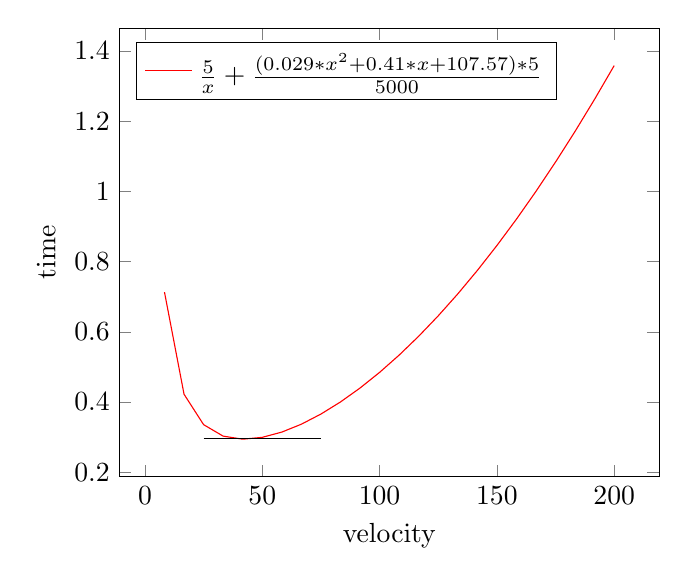
\begin{tikzpicture}
\begin{axis}[xlabel=velocity, ylabel=time,legend style={legend pos=north west}]
\addplot[draw=red,domain=0:200]{(5/x)+(((0.0286*x^2 + 0.4096*x + 107.57)*5)/5000)};
\addlegendentry{$\frac{5}{x}+\frac{(0.029*x^2 + 0.41*x + 107.57)*5}{5000}$}

\addplot[draw=black,domain=25:75]{0.295};
% \addplot[mark=*, domain=25:75] coordinates {(37,295)};
\end{axis}
\end{tikzpicture}% 
\caption{In this instance of $T(v,(u_1, u_2))$, going from $u_1$ to $u_2$, we have a distance of $5 \si{\km}$ and a charge speed of $5 \si{\kW}$ on $u_1$. The optimal speed in this case is $42.12\si{\km\per\hour}$, and the total time is roughly 17 minutes to pass through the edge when driving and charging}
\end{figure}
Having the two ways of deciding the time it takes to pass an edge a algorithm can be created which decide how to drive each road segment can be formulated.   

\begin{algorithmic}
\Function{GreedyHeuristic}{$RN,s,t,EV$}
	\ForAll{$v \in RN.V$} 
		\State $v.time = \infty$
		\State $v.predecessor = NIL$
		\State $v.preCS = NIL$
		\State $v.B_{cur} = 0$
	\EndFor
	\State $s.time = 0$
	\State $s.B_{cur} = EV.B_{cur}$

	\State $Q = PriorityQueue$
	\State $insert(Q, (s.time, s))$	
	\While{$Q \neq \emptyset$} 
		\State $u = extractmin(Q)$
		\ForAll{$v \in RN.adj(u)$} 
			\State $time,preCS,B_{cur},energy = $
			\State $travel\_time(RN, u, v, EV)$
			\If{$v.time > u.time + time$} 
				\State $v.time = u.time + time$
				\State $v.predecessor = u$
				\State $v.B_{cur} = B_{cur}$
				\State $v.preCS = preCS$
				\State $insert(Q, (v.time, v))$	
			\EndIf
			\If{ $preCS \neq NIL$}
				\State $a$
			\EndIf
		\EndFor
	\EndWhile
	\State \Return $t.time, t.path$
\EndFunction
\end{algorithmic}\label{alg:fastest_path}

\begin{algorithmic}
\Function{travel\_time}{$RN, u, v, EV$}
	\State $e = (u, v)$
	\State $v_{opt1} = solve1\langle v, EV.B_{cur}-RN.D(e)*EV.R_{CO}(v) = 0\rangle$
	\If{$ u.B_{cur} - RN.D(e)*EV.R_{CO}(v_{opt1}) < 0 $}
		\State $time_1 = \infty$
	\Else
		\State $time_1 = RN.D(e) / v_{opt1}$
		\State $energy\_used_{1} = RN.D(e)*EV.R_{CO}(v_{opt1})$
	\EndIf
		\State $CS = getCS(u, v)$ 
		\State $energy\_needed_{2} = \infty$
		\State $energy = u.B_{cur}$
		\State $time\_added = 0$
		\State $time_2 = \infty$
	\While{$energy\_needed_{2} > energy  \And  len(CS) \neq 0$}
		\State $best_{CS} = extractmax(CS)$
		\State $B_{possible} = best_{CS}.B_{possible}$
		\State $charge\_rate = RN.R_{CH}(best_{CS})$
		\State $v_{opt2} = solve2 \langle v, B_{possible},  RN.D(e)/v + $
			\State $(RN.D(e)*EV.R_{CO}(v)-energy)/charge\_rate) \rangle$
		\State $energy\_needed_{2} = RN.D(e)*EV.R_{CO}(v_{opt2})$
		\State $energy = energy + B_{possible}$
		\If{$v_{opt2} == \infty$}
			\State $time\_added = time\_added + B_{possible}/charge\_rate$
			\State $CS.remove(0)$
			\State $updateCS(CS)$
		\EndIf	
	\EndWhile
	\If{$v_{opt2} \neq \infty$}
		\State $time_2 = RN.D(e)*EV.R_{CO}(v_{opt2}) + $
		\State $energy\_needed_{2}/charge\_rate + time\_added$
		\State $energy\_used_2 = RN.D(e)*EV.R_{CO}(v_{opt2})$
	\EndIf
	\If{$time_1 <= time_2$}
		\State \Return $time_1, CS, energy\_used_1$
	\ElsIf{$time_1 > time_2$}
		\State \Return $time_2, CS, energy\_used_2$
	\Else
		\State \Return $\infty, NIL, \infty$
	\EndIf

\EndFunction
\end{algorithmic}\label{alg:fastest_path}

The worst case running time of the greedy heuristic algorithm is bound by three procedures. First there is the main procedure that is derived directly from Dijkstra's, which have a worst case of $O(V^2)$ on dense graphs. To that we need to multiply $O(V)$ from the travel\_time procedure, as this procedure might go through all vertices, if the vehicle is set to charge at a new charging station for every found edge and every vertex in the graph is also a charging station. Finally we have the procedure that maintain a set of charging stations relevant on each vertex. In the special case where the vehicle have an infinitely large battery capacity, but start without any battery, and every vertex found happens to be a charging station with a charge rate in a decreasing order, the procedure would have to multiply $O(V)$ to the worst case.
However only one of the last two procedure's $O(V)$ complexity is added, as the case where the algorithm chose to charge at a new charge station for every edge never happens with an infinity large battery. Likewise the case where the procedure maintain a list of every charging station, never happens if the car has a limited battery capacity. Resulting in a worst case running time of $O(V^3)$.

In practice Dijkstra's algorithm run faster on a sparse graph, which road networks are, and both of the remaining procedures are simultaneously limited from the fact that only a small amount of charging stations exist and that EV battery capacity is limited.
\todo[inline]{need proof-reading}



